\documentclass[assignment = 2]{homework}

\usepackage{caption, subcaption, pdfpages, float}
\usepackage{graphics, wrapfig, pgf, graphicx}
\usepackage{enumitem}
\graphicspath{{../}}


% pacotes para importar código
\usepackage{caption, booktabs}
\usepackage[section, newfloat]{minted}
\definecolor{sepia}{RGB}{252,246,226}
\setminted{
    bgcolor = sepia,
    style   = pastie,
    frame   = leftline,
    autogobble,
    samepage,
    python3,
}
\setmintedinline{
    bgcolor={}
}

% ambientes de códigos de Python
\newmintedfile[pyinclude]{python}{}
\newmintinline[pyline]{python}{}
\newcommand{\pyref}[2]{\href{#1}{\texttt{#2}}}

% \SetupFloatingEnvironment{listing}{name=Código}
% \captionsetup[listing]{position=below,skip=-1pt}

\usepackage{csquotes}
\usepackage[style=verbose-ibid,autocite=footnote,notetype=foot+end,backend=biber]{biblatex}
\addbibresource{referencias.bib}
\usepackage[section]{placeins}

\usepackage[hidelinks]{hyperref}
\usepackage[noabbrev, nameinlink, brazilian]{cleveref}
\hypersetup{
    pdftitle  = {MC920 - Trabalho 2 - 187679},
    pdfauthor = {Tiago de Paula}
}

\newcommand{\textref}[2]{
    \hyperref[#2]{#1 \ref*{#2}}
}

\usepackage{import}
\usepackage{tikz}
\usetikzlibrary{matrix}
\usetikzlibrary{positioning}

\newenvironment{kmatrix}{
    \begin{tikzpicture}[node distance=0cm]
        \tikzset{square matrix/.style={
                matrix of nodes,
                column sep=-\pgflinewidth, row sep=-\pgflinewidth,
                nodes={draw,
                    minimum height=0.7cm,
                    anchor=center,
                    text width=0.7cm,
                    align=center,
                    inner sep=0pt
                },
            },
            square matrix/.default=0.7cm
        }
}{
    \end{tikzpicture}%
}

\newcommand*{\Scale}[2][4]{\scalebox{#1}{\ensuremath{#2}}}%

\newcommand{\red}[1]{\textcolor{red}{\textbf{#1}}}

\begin{document}

    \pagestyle{main}

    \section{Introdução}

Este trabalho teve como objetivo a implementação de técnicas de pontilhado com difusão de erros. A ideia é reduzir a quantidade de cores tentando manter a imagem o mais próximo possível da original. Isso é feito reduzindo a intesidade para seu limite mais próximo, ao longo de um caminho pela imagem, mas aplicando uma distribuição de erros na vizinhança do pixel.

A \cref{fig:base} apresenta as imagens base deste trabalho, usadas para análise e discussão das formas diferentes de aplicar o pontilhado. As figuras \ref{fig:baboon} e \ref{fig:peppers} são $512 \times 512$, enquanto a \cref{fig:monalisa} é $256 \times 256$ e a \cref{fig:watch} é $1024 \times 768$. Ao todo serão aplicadas 6 distribuições de erro com \red{2 curvas} diferentes. As distribuições de erros serão apresentadas ao longo do relatório, na \red{seção ??}, equanto as curvas podem ser encontradas na \red{seção ??}.

\begin{figure}[H]
    \centering
    \begin{subfigure}{0.33\textwidth}
    \centering
    \includegraphics[width=4.4cm]{imagens/baboon.png}
    \caption{\texttt{imagens/baboon.png}}
    \label{fig:baboon}
\end{subfigure}%
\begin{subfigure}{0.33\textwidth}
    \centering
    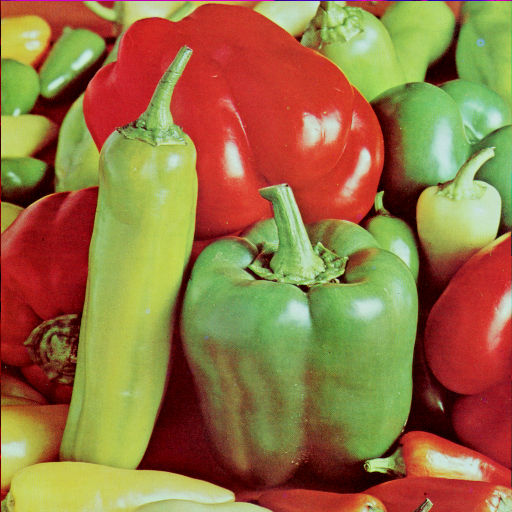
\includegraphics[width=4.4cm]{imagens/peppers.png}
    \caption{\texttt{imagens/peppers.png}}
    \label{fig:peppers}
\end{subfigure}\\[8pt]
\begin{subfigure}{0.33\textwidth}
    \centering
    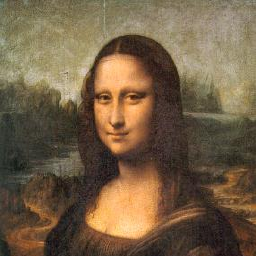
\includegraphics[width=4.4cm]{imagens/monalisa.png}
    \caption{\texttt{imagens/monalisa.png}}
    \label{fig:monalisa}
\end{subfigure}%
\begin{subfigure}{0.33\textwidth}
    \centering
    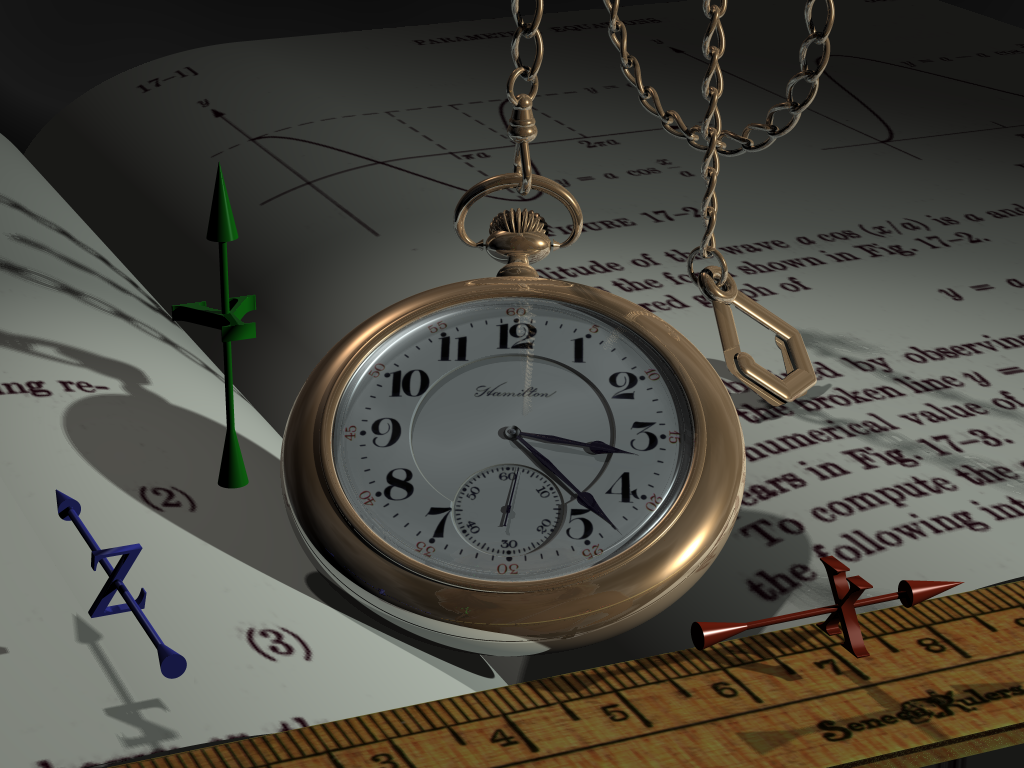
\includegraphics[width=4.4cm]{imagens/watch.png}
    \caption{\texttt{imagens/watch.png}}
    \label{fig:watch}
\end{subfigure}

    \caption{Imagens base da comparação dos filtros.}
    \label{fig:base}
\end{figure}


    \section{O Programa}

Além das bibliotecas padrão de Python, foram utilizados os pacotes NumPy \autocite{ref:numpy} e, de forma opcional, Numba \autocite{ref:numba}.

\subsection{Código Fonte}

    O programa foi desenvolvido em Python 3.8, mas deveria funcionar com a versões 3.7 e 3.9 também. Além disso, o código fonte foi separado nos seguintes arquivos:

    \begin{description}
        \item[main.py] É o corpo do programa, resposável por processar os comandos e as opções da linha de comando.

        \item[lib] Pacote interno com as operações de pontilhado.

        \begin{description}
            \item[lib/\_\_init\_\_.py] Função geral de aplicação do pontilhado em imagens coloridas e em escala de cinza, com as opções de varredura.

            \item[lib/nb.py] Mock up do decorador \mintinline{python3}{@numba.jit} \autocite{ref:numbajit}, para que a ferramenta funcione tanto com ou sem a biblioteca Numba.

            \item[lib/horizontal.py] Implementação das varreduras horizontais, tanto a varredura unidirecional quanto a alternada.

            \item[lib/direcao.py] Controle de direção para varreduras não horizontais (espiral e curvas de Hilbert).

            \item[lib/espiral.py] Implementação da varredura em espiral.

            \item[lib/hilbert.py] Varredura seguindo uma curva de Hilbert.
        \end{description}

        \item[dists.py] Definição das distribuições de erro ao longo da operação de meios-tons.

        \item[inout.py] Funções que tratam da entrada e saída do programa, como leitura e escrita de arquivos de imagem e também da apresentação da imagem em uma janela gráfica.

        \item[tipos.py] Definição de alguns tipos para checagem estática com \texttt{mypy} \autocite{ref:mypy}.
    \end{description}

    Todas as figuras base utilizadas neste relatório podem ser encontradas na pasta \texttt{imagens} do código fonte, como descrito nos rótulos da \cref{fig:base}. Além disso, foi disponibilizado também um \textit{script} em \texttt{bash}, \texttt{run.sh}, que realiza todos os processamentos requeridos em cada uma das imagens na pasta.

\subsection{Execução} \label{sec:execucao}

    A execução deve ser feita através do interpretador de Python 3.7+. A única entrada obrigatória é o caminho para a imagem PNG que será processada. Ao final da execução, a imagem resultante será exibida na tela.

    \begin{figure}[H]
        \centering
        \includegraphics[width=6cm]{resultados/execucao.png}

        \caption{Aplicação de pontilhado com a \texttt{baboon.png}.}
        \label{fig:execucao}
    \end{figure}

    Os argumentos opicionais podem ser vistos com \mintinline{bash}{$ python3 main.py --help}. A mais importante das opções é \mintinline{text}{--output}, ou \mintinline{text}{-o}, que salva o resultado em um arquivo PNG em vez de exibir na tela. Se é desejável tanto a exibição da imagem quanto o salvamento no arquivo, o argumento \mintinline{text}{--force-show} ou \mintinline{text}{-f} pode ser usado. Também existe a opção \mintinline{bash}{--grayscale} ou \mintinline{bash}{-g} que faz o processamento em escala de cinza.

    As outras opções são referentes à técnica de pontilhado. A flag \mintinline{bash}{--varedura} ou \mintinline{bash}{-v} controla o forma de varrredura na image, como descrito na \ref{sec:varredura}. A distribuição de erros aplicada pode ser modificada com \mintinline{bash}{--destribuicao} ou \mintinline{bash}{-d} e aceita o nome de qualquer um de seus idealizadores.

    Por exemplo, o comando abaixo apresenta a \cref{fig:execucao} em uma nova janela gráfica.

    \begin{minted}{bash}
        $ python3 main.py imagens/baboon.png -g -d ninke
    \end{minted}

\subsection{A biblioteca Numba}

    A ferramenta foi desenvolvida com requerimento mínimo sendo apenas o NumPy. No entanto, se presente, a biblioteca Numba causa um grande diferencial no tempo de execução das técnicas de pontilhado (mais de trinta vezes mais rápido, na máquina de desenvolvimento). Por isso, ela é fortemente recomendada na execução do código.


    \section{Implementação} \label{sec:impl}

\subsection{Técnica de Meios-Tons com Difusão de Erro}

    Essa técnica de pontilhado se baseia em alterar cada pixel com escala de 8 bits para escala de 2 bits, levando para o seu bit mais próximo. No entanto, ao longo do processo, o erro é calculado em relação ao novo pixel, que é então distribuído na sua vizinhaça, influenciando as aplicações nos pixels seguintes.

    Assim, quando um pixel resulta em valor muito distante do original, seus vizinhos são reduzidos ou incrementados, aumentando a chance de que eles sejam transformados para outro nível. Isso faz com que a vizinhaça mantenha um pouco mais da distribuição local de intensidade, fazendo com que imagem fique similar à original para o nosso sistema visual.

    A distribuição de erros pode ser feita de várias formas, como pode ser visto na \cref{sec:resultado}.

\subsection{Formas de Varredura} \label{sec:varredura}

    A técnica de pontilhado com distribuição de erros altera a imagem enquanto é aplicada, o que faz com que o caminho escolhido altere o resultado. Por isso, o pontilhado foi implementado seguindo quatro formas de varredura, apresentadas na \cref{fig:varredura}. Apesar disso, as varreduras que serão mais discutidas aqui serão a unidirecional (\ref{fig:varredura:unidirecional}) e a alternada (\ref{fig:varredura:alternada}).

    \begin{figure}[H]
        \centering
        \newcommand{\imagem}[1]{
    \centering
    \begin{subfigure}{0.32\textwidth}
        \centering
        \includegraphics[width=4.4cm]{imagens/#1.png}
        \caption{\texttt{figuras/#1.png}}
        \label{fig:#1:orig}
    \end{subfigure}%
    \begin{subfigure}{0.32\textwidth}
        \centering
        \includegraphics[width=4.4cm]{resultados/var/unidir_#1.png}
        \caption{Varredura unidirecional.}
        \label{fig:#1:unidir}
    \end{subfigure}%
    \begin{subfigure}{0.32\textwidth}
        \centering
        \includegraphics[width=4.4cm]{resultados/var/alternada_#1.png}
        \caption{Varredura alternada.}
        \label{fig:#1:alt}
    \end{subfigure}
}

\begin{figure}[H]
    \centering
    \imagem{baboon}\\[8pt]
    \imagem{peppers}\\[8pt]
    \imagem{monalisa}\\[8pt]
    \imagem{watch}

    \caption{Aplicação da distribuição de Floyd e Steinberg com as duas varreduras.}
    \label{fig:resultado:varredura}
\end{figure}

Na \cref{fig:resultado:varredura}, os resultados das duas varreduras são visualmente muito semelhantes e asmétricas da \cref{tab:varedura} corroboram com essa ideia, mostrando uma variação pequena de uma opção para a outra. A maior diferença visual aparece na imagem \texttt{peppers.png}, onde a varredura unidirecional (\ref{fig:peppers:unidir}) gera pequenos artefatos em formato de linhas horizontais, principalmente no pimentão vermelho.

\begin{table}[H]
    \centering
    \caption{Comparativo entre os resultados da \cref{fig:resultado:varredura}.}
    \label{tab:varedura}

    \begin{tabular}{cc|cccc}
        \toprule
        Figura & Varredura & RMSE & SNR (dB) & PSNR (dB) & Correlação \\
        \midrule
        \multirow{2}{*}{\texttt{baboon.png}} & Unidirecional & 10.367 & -0.004 & 27.818 & 0.480 \\
        & Alternada & 10.364 & -0.001 & 27.820 & 0.477 \\
        \midrule
        \multirow{2}{*}{\texttt{peppers.png}} & Unidirecional & 10.322 & -0.017 & 27.856 & 0.531 \\
        & Alternada & 10.325 & -0.020 & 27.853 & 0.531 \\
        \midrule
        \multirow{2}{*}{\texttt{monalisa.png}} & Unidirecional & 10.411 & 0.009 & 27.781 & 0.419 \\
        & Alternada & 10.407 & 0.013 & 27.784 & 0.418 \\
        \midrule
        \multirow{2}{*}{\texttt{watch.png}} & Unidirecional & 10.262 & 0.016 & 27.907 & 0.372 \\
        & Alternada & 10.263 & 0.015 & 27.905 & 0.371 \\
        \bottomrule
    \end{tabular}
\end{table}

Nos resultados seguintes, a imagens serão varridas de forma alternada, como este é o padrão da ferramenta.


        \caption{Argumentos válidos para \mintinline{bash}{--varredura} ou \mintinline{bash}{-v}.}
        \label{fig:varredura}
    \end{figure}

    Para a varrudura alternada, a distribuição é aplicada em duas orientações, normal e invertida horizontalmente, enquanto para as curvas em espiral e de Hilbert a distribuição dois considerada em quatro orientações, seguindo rotações sucessivas de 90\textdegree{} na matriz.

    % \begin{figure}
    %     \centering
    %     \begin{subfigure}{0.30\textwidth}
    \centering
    \begin{kmatrix}
    \matrix[square matrix]{
        ~ & $f(x, y)$ & 7/16 \\
        3/16 & 5/16 & 1/16 \\
    };
\end{kmatrix}
    \caption{Floyd e Steinberg}
\end{subfigure}%
\begin{subfigure}{0.63\textwidth}
    \centering
    \begin{kmatrix}
    \matrix[square matrix]{
        ~ & ~ & ~ & $f(x, y)$ & ~ & $\displaystyle\frac{32}{200}$ & ~ \\
        $\displaystyle\frac{12}{200}$ & ~ & $\displaystyle\frac{26}{200}$ & ~ & $\displaystyle\frac{30}{200}$ & ~ & $\displaystyle\frac{16}{200}$ \\
        ~ & $\displaystyle\frac{12}{200}$ & ~ & $\displaystyle\frac{26}{200}$ & ~ & $\displaystyle\frac{12}{200}$ & ~ \\
        $\displaystyle\frac{5}{200}$ & ~ & $\displaystyle\frac{12}{200}$ & ~ & $\displaystyle\frac{12}{200}$ & ~ & $\displaystyle\frac{5}{200}$ \\
    };
\end{kmatrix}
    \caption{Stevenson e Arce}
\end{subfigure}\\[8pt]
\begin{subfigure}{0.48\textwidth}
    \centering
    \begin{kmatrix}
    \matrix[square matrix]{
        ~ & ~ & $f(x, y)$ & 8/32 & 4/32 \\
        2/32 & 4/32 &  8/32 & 4/32 & 2/32 \\
    };
\end{kmatrix}
    \caption{Burkes}
\end{subfigure}%
\begin{subfigure}{0.48\textwidth}
    \centering
    \begin{kmatrix}
    \matrix[square matrix]{
        ~ & ~ & $f(x, y)$ & 5/32 & 3/32 \\
        2/32 & 4/32 &  5/32 & 4/32 & 2/32 \\
        ~ & 2/32 &  3/32 & 2/32 & ~ \\
    };
\end{kmatrix}
    \caption{Sierra}
\end{subfigure}\\[8pt]
\begin{subfigure}{0.48\textwidth}
    \centering
    \begin{kmatrix}
    \matrix[square matrix]{
        ~ & ~ & $f(x, y)$ & 8/42 & 4/42 \\
        2/42 & 4/42 &  8/42 & 4/42 & 2/42 \\
        1/42 & 2/42 &  4/42 & 2/42 & 1/42 \\
    };
\end{kmatrix}
    \caption{Stucki}
\end{subfigure}%
\begin{subfigure}{0.48\textwidth}
    \centering
    \begin{kmatrix}
    \matrix[square matrix]{
        ~ & ~ & $f(x, y)$ & 7/48 & 5/48 \\
        3/48 & 5/48 & 7/48 & 5/48 & 3/48 \\
        1/48 & 3/48 & 5/48 & 3/48 & 1/48 \\
    };
\end{kmatrix}
    \caption{Jarvis, Judice e Ninke}
\end{subfigure}
    % \end{figure}


\end{document}
